\chapter{Resultados}\label{cap:resultados}

Este capítulo apresenta e discute os resultados obtidos com os módulos intervencionados. O termo de comparação é a solução de referência do desafio SoccerNet-GSR \citep{somers2024soccernet}, executada por nós com os seus módulos originais, incluindo o leitor de números MMOCR, nos mesmos vídeos e no mesmo ambiente em que correu o sistema proposto. Como os dois sistemas partilham a deteção, o seguimento e as representações de reidentificação, os \emph{tracklets} avaliados são os mesmos e qualquer diferença resulta apenas do que foi alterado. A avaliação abrange os três subconjuntos anotados, teste com $49$ vídeos, validação com $53$ e treino com $57$, num total de $159$ sequências; a sequência SNGS-096 do conjunto de validação não pôde ser processada por uma falha do módulo de calibração, comum aos dois sistemas.

Apresentam-se primeiro os resultados de cada módulo isoladamente, com métricas dedicadas e com a inspeção visual descrita na Secção~\ref{sec:protocolo}, e depois o seu efeito no sistema completo, medido pelo GS-HOTA. Recorde-se, da Secção~\ref{sec:ambiente}, que o conjunto de treino não interveio em nenhuma decisão de conceção e funciona neste trabalho como conjunto de retenção.

\section{Reconhecimento de Número de Camisola}\label{sec:res_jnr}

O reconhecimento do número de camisola é avaliado pela exatidão por \emph{tracklet}, calculada por correspondência (IoU $\geq 0.30$) entre as deteções e a anotação de referência, sobre os \emph{tracklets} de jogadores com número anotado e suficientemente consistentes para excluir a influência de trocas de identidade do \emph{tracker}. A solução de referência e o sistema proposto são avaliados da mesma forma, com o mesmo limiar de correspondência e a mesma anotação, sobre exatamente os mesmos \emph{tracklets}, pelo que os denominadores coincidem e a comparação é direta.

\subsection{Resultados}\label{sec:res_jnr_resultados}

Os valores apresentados correspondem ao sistema final, com a decisão pela confiança da leitura descrita na Secção~\ref{sec:met-jnr-confianca}; a Secção~\ref{sec:res_jnr_confianca} compara-o com a primeira versão do módulo. A Tabela~\ref{tab:jnr} resume os resultados. Nos três subconjuntos, a exatidão do reconhecimento mais do que duplica, de $19.2\%$ para $46.8\%$ no teste, de $15.8\%$ para $41.8\%$ na validação e de $12.0\%$ para $39.8\%$ no treino, o que sobre a totalidade dos $159$ vídeos corresponde a uma subida de $15.3\%$ para $42.6\%$. O ganho no conjunto de treino, que nunca interveio no desenvolvimento, é da mesma ordem do obtido no conjunto de teste, sobre o qual o módulo foi afinado.

\begin{table}[htbp]
    \centering
    \caption{Exatidão do reconhecimento do número de camisola, por \emph{tracklet}, sobre os mesmos \emph{tracklets} nos dois sistemas.}
    \label{tab:jnr}
    \begin{tabular}{|l|c|c|c|}
        \hline
        \textbf{Conjunto} & \textbf{Referência (MMOCR)} & \textbf{Proposto (Qwen2.5-VL)} & \textbf{$\Delta$} \\
        \hline
        Teste ($49$ vídeos)     & $19.2\%$ ($333/1731$)   & $46.8\%$ ($810/1731$)   & $+27.6$ pp \\
        \hline
        Validação ($53$ vídeos) & $15.8\%$ ($267/1691$) & $41.8\%$ ($707/1691$) & $+26.0$ pp \\
        \hline
        Treino ($57$ vídeos)    & $12.0\%$ ($265/2216$) & $39.8\%$ ($882/2216$) & $+27.8$ pp \\
        \hline
        Total ($159$ vídeos)    & $15.3\%$ ($865/5638$)     & $42.6\%$ ($2399/5638$)     & $+27.2$ pp \\
        \hline
    \end{tabular}
\end{table}

A distribuição dos ganhos por vídeo (Tabela~\ref{tab:jnr-distribuicao} e painel superior da Figura~\ref{fig:delta-video}) mostra que a melhoria não se concentra num punhado de casos. O sistema proposto melhora em $156$ dos $159$ vídeos, com um ganho mediano de $27.3$ pontos percentuais. Empata em três (SNGS-042, SNGS-045 e SNGS-049) e não regride em nenhum. Na solução de referência, quatro vídeos não têm uma única leitura correta e apenas dois atingem os $50\%$ de exatidão. No sistema proposto nenhum vídeo fica sem leituras corretas e $50$ atingem ou ultrapassam esse valor.

\begin{table}[htbp]
    \centering
    \caption{Distribuição dos ganhos do reconhecimento do número de camisola sobre a solução de referência ($159$ vídeos).}
    \label{tab:jnr-distribuicao}
    \begin{tabular}{|l|c|}
        \hline
        \textbf{Ganho face à referência} & \textbf{N.º de vídeos} \\
        \hline
        Superior a $+40$ pp & $20$ \\
        \hline
        De $+30$ a $+40$ pp & $45$ \\
        \hline
        De $+20$ a $+30$ pp & $48$ \\
        \hline
        De $+10$ a $+20$ pp & $38$ \\
        \hline
        De $+1$ a $+10$ pp  & $5$ \\
        \hline
        Empate ($\pm 1$ pp) & $3$ \\
        \hline
        Regressão           & $0$ \\
        \hline
    \end{tabular}
\end{table}


\subsection{Teto da Abordagem}\label{sec:res_jnr_teto}

Alcançado o ganho da primeira versão do módulo, restava perceber onde residiam os limites da abordagem. Para isso, testaram-se três abordagens de melhoria num conjunto de controlo de seis vídeos (os quatro com piores resultados e dois em que o sistema já funcionava bem), sob a premissa de resolver os casos falhados sem prejudicar os bem-sucedidos.

A primeira abordagem atribuiu a cada recorte uma pontuação de qualidade, calculada a partir da nitidez da imagem, da área do recorte e do número de recortes que sustentavam a leitura na janela temporal. Na votação, as leituras com maior pontuação passaram a ter mais peso. O resultado foi um ganho residual e inconsistente, sem qualquer alteração nos vídeos mais problemáticos. A segunda, um realce de contraste por CLAHE (\emph{Contrast Limited Adaptive Histogram Equalization}) aplicado aos recortes antes da leitura pelo VLM, teve um impacto claramente negativo, degradando mais vídeos do que aqueles que melhorou. A terceira, a apresentação de todas as vistas de um \emph{tracklet} numa única imagem composta em grelha, permitindo ao modelo agregar a evidência internamente em vez de recorrer à votação temporal externa, também não produziu melhorias.

O diagnóstico foi o mesmo nas três experiências. Nos casos difíceis, o modelo falha a leitura porque a informação não está presente nos \emph{pixels}, seja pela distância da câmara, seja pela orientação do jogador, e nenhuma reponderação heurística, ajuste de contraste ou recombinação de vistas cria informação onde ela não existe. O que estas experiências não resolviam era outro problema. O sistema não sabia distinguir as leituras em que o modelo tinha visto o número das leituras em que o tinha adivinhado. Essa informação não estava na imagem, estava no próprio modelo. Usá-la na decisão (Secção~\ref{sec:res_jnr_confianca}) foi o que permitiu reduzir o erro sem alterar a leitura.

\subsection{Controlo pela Confiança da Leitura}\label{sec:res_jnr_confianca}

A exatidão por \emph{tracklet} da Tabela~\ref{tab:jnr} trata todos os \emph{tracklets} por igual. O GS-HOTA, pelo contrário, conta deteções, e um \emph{tracklet} longo com o número errado pesa tanto como muitos \emph{tracklets} curtos juntos. Para perceber onde estava o custo do número na métrica oficial, as deteções de jogadores emparelhadas com a anotação foram classificadas em cinco categorias, conforme a anotação tem ou não número e o sistema atribui ou não um número (Tabela~\ref{tab:jnr-categorias}).

Na primeira versão do módulo, sobre os $159$ vídeos, $51.4\%$ das deteções recebiam o número certo, $12.3\%$ recebiam um número errado e $2.5\%$ recebiam um número quando o jogador não tinha número visível na anotação. A maior parte do erro estava em \emph{tracklets} longos, já que $9.2\%$ de todas as deteções pertenciam a \emph{tracklets} com mais de $200$ \emph{frames} que terminavam com um número errado. Os registos de execução guardam os votos de cada janela, o que permitiu reconstituir cada decisão. Em cerca de um terço das deteções com número errado, o número certo chegou a ser lido, mas perdeu a votação para leituras erradas mais numerosas. Nas restantes, o número certo nunca foi lido, e as leituras erradas vinham de recortes em que o número não era legível. Em ambos os casos, o que faltava à decisão era saber quais das leituras eram seguras.

A regra de decisão pela confiança (Secção~\ref{sec:met-jnr-confianca}) foi testada primeiro numa amostra aleatória de $10$ vídeos de teste e validação. Como a tendência se confirmou, foi alargada por fases, sempre com vídeos sorteados, até cobrir os $159$. Em cada fase, a primeira versão e a versão com confiança foram comparadas sobre as mesmas deteções, com a mesma anotação e com o GS-HOTA oficial. A Tabela~\ref{tab:jnr-categorias} resume o resultado.

\begin{table}[htbp]
    \centering
    \caption{O que acontece às deteções de jogadores, em percentagem, na primeira versão do módulo e com a decisão pela confiança da leitura ($159$ vídeos).}
    \label{tab:jnr-categorias}
    \begin{tabular}{|l|c|c|c|}
        \hline
        \textbf{Categoria} & \textbf{Primeira versão} & \textbf{Com confiança} & \textbf{$\Delta$} \\
        \hline
        Número certo                               & $51.4$ & $57.0$ & $+5.6$ \\
        \hline
        Número errado                              & $12.3$ & $4.4$  & $-7.9$ \\
        \hline
        Número atribuído sem número na anotação    & $2.5$  & $0.5$  & $-2.0$ \\
        \hline
        Sem número, e a anotação também não tem    & $10.9$ & $12.9$ & $+2.0$ \\
        \hline
        Sem número, mas a anotação tem             & $22.9$ & $25.2$ & $+2.3$ \\
        \hline
    \end{tabular}
\end{table}

O efeito principal é a redução dos números errados para cerca de um terço, de $12.3\%$ para $4.4\%$ das deteções, e dos números atribuídos a jogadores sem número de $2.5\%$ para $0.5\%$. Ao mesmo tempo, o número certo sobe $5.6$ pontos percentuais. À primeira vista, uma regra mais conservadora não deveria acertar mais. A explicação está no filtro de qualidade, agora mais permissivo. Como a confiança trava as leituras inseguras, foi possível aceitar recortes mais pequenos e menos nítidos, e parte deles tem um número legível que a primeira versão nem chegava a ver. O custo é o previsto no desenho da regra. Os jogadores que ficam sem número apesar de o terem aumentam $2.3$ pontos, sobretudo casos em que o modelo leu o número certo em várias janelas, mas sempre com confiança abaixo do limiar.

No GS-HOTA oficial, a subida é consistente nos três subconjuntos, incluindo o de treino, que não interveio em nenhuma decisão (Tabela~\ref{tab:jnr-confianca-gshota}), e faz-se sobretudo pela componente de deteção (DetA).

\begin{table}[htbp]
    \centering
    \caption{GS-HOTA oficial com a primeira versão do módulo e com a decisão pela confiança da leitura, sobre os mesmos vídeos.}
    \label{tab:jnr-confianca-gshota}
    \begin{tabular}{|l|c|c|c|}
        \hline
        \textbf{Conjunto} & \textbf{Primeira versão} & \textbf{Com confiança} & \textbf{$\Delta$} \\
        \hline
        Teste ($49$ vídeos)     & $43.76$ & $47.87$ & $+4.10$ \\
        \hline
        Validação ($53$ vídeos) & $35.13$ & $36.79$ & $+1.66$ \\
        \hline
        Treino ($57$ vídeos)    & $42.79$ & $45.37$ & $+2.58$ \\
        \hline
    \end{tabular}
\end{table}

A melhoria não é uniforme. O GS-HOTA sobe em $120$ dos $159$ vídeos e desce em $27$. Destes, $13$ descem menos de um ponto e $9$ descem mais de dois. A inspeção dos casos com maior descida mostra dois padrões. No primeiro, o modelo lê o número certo várias vezes, mas sempre com pouca confiança. No SNGS-056, um jogador com o número 14 foi lido como 14 em nove de doze janelas, todas com confiança entre $0.3$ e $0.43$, e ficou sem número, quando a primeira versão o acertava. É o custo direto do limiar. No segundo, a descida resulta da própria anotação. No SNGS-188, um \emph{tracklet} lido como 14 com confiança entre $0.6$ e $0.8$ em quase todas as janelas está emparelhado com um jogador anotado com o número 34, e os recortes mostram de forma legível um 14. Casos semelhantes de anotação incompleta ou inconsistente foram encontrados noutros vídeos, em que um número claramente visível não consta da anotação.

No extremo oposto, o SNGS-196 ilustra o comportamento pretendido. Na primeira versão, $9\%$ das deteções recebiam o número certo e $16\%$ um número errado. Com a decisão pela confiança, o número certo sobe para $50\%$, o número errado desaparece e o GS-HOTA do vídeo passa de $17.1$ para $38.7$. Dos quinze jogadores cujo número muda, doze que estavam sem número passam a ter o número certo, dois números errados são corrigidos e um terceiro é retirado. Nenhum jogador que estava correto passa a errado.

\subsection{Alternativas Testadas e Rejeitadas}\label{sec:res_jnr_rejeitadas}

Antes e depois de chegar à decisão pela confiança, foram avaliadas outras formas de reduzir o erro do número. Todas foram medidas com o mesmo critério, o GS-HOTA oficial por subconjunto e vídeo a vídeo, e só seriam aceites se não piorassem nenhum dos indicadores de erro. Nenhuma cumpriu esse critério.

\medskip\noindent\textbf{Fusão de fragmentos do seguimento.} Um mesmo jogador é frequentemente dividido pelo \emph{tracker} em vários \emph{tracklets}, alguns dos quais demasiado curtos para serem lidos. Juntar fragmentos da mesma equipa que nunca coexistem no tempo e são próximos no espaço de reidentificação, propagando o número do fragmento mais confiante, aumentou a exatidão por \emph{tracklet} em $5.5$ pontos percentuais. O GS-HOTA subiu apenas $0.04$ pontos. Os fragmentos corrigidos eram quase todos curtos e representavam poucas deteções, e as fusões erradas degradavam a associação entre identidades.

\medskip\noindent\textbf{Regras de decisão alternativas.} Somar as confianças de cada número, em vez de contar as janelas confiantes, não superou a regra final. Uma regra híbrida tentou recuperar os casos de leitura certa com pouca confiança. Quando nenhuma janela era confiante, usava a decisão da primeira versão, desde que pelo menos duas janelas concordassem. Numa amostra de $20$ vídeos não trouxe ganho no GS-HOTA face à regra final e, no conjunto de teste, voltou a atribuir números a jogadores sem número, que passaram de $0.1\%$ para $1.1\%$ das deteções.

\medskip\noindent\textbf{Unicidade do número dentro da equipa.} Dois jogadores da mesma equipa não podem ter o mesmo número em campo ao mesmo tempo. A inspeção visual mostrou casos em que esta regra é violada, como no SNGS-196, em que um \emph{tracklet} perde o jogador que seguia, reaparece colado a outro jogador da mesma equipa e leva consigo o número do primeiro. Testaram-se duas formas de impor a regra. A primeira retira o número ao \emph{tracklet} mais fraco nos \emph{frames} em que dois \emph{tracklets} da mesma equipa partilham o número. A segunda, mais restrita, só o faz quando os dois estão a mais de $5$~m de distância no campo, e retira o número ao que apareceu mais recentemente. Numa primeira contagem, em $60$ vídeos, encontraram-se $107$ conflitos. Em $68$ deles os dois \emph{tracklets} estavam corretos. Era o mesmo jogador, dividido em dois \emph{tracklets} que se sobrepunham durante alguns \emph{frames}. As duas versões, medidas em $117$ dos $159$ vídeos, deixaram o GS-HOTA igual ou mais baixo nos três subconjuntos, com descidas até $0.15$ pontos, e pioraram mais de vinte vídeos. Mesmo no SNGS-196, retirar o número ao troço errado baixou o GS-HOTA do vídeo, porque a métrica penaliza uma identidade cujo número muda a meio mais do que ganha no troço corrigido. O erro de fundo é uma troca de identidade do seguimento, e não se corrige do lado do número sem alterar o \emph{tracker}, que está fora do âmbito deste trabalho.

\medskip\noindent\textbf{Lição sobre a métrica.} Estas experiências mostram que ganhos medidos por \emph{tracklet} não se traduzem necessariamente em ganhos no GS-HOTA, que pondera por deteção e avalia a coerência das identidades ao longo do tempo. Uma correção que atue sobre \emph{tracklets} curtos é praticamente invisível na métrica oficial, e uma correção que altere o número de parte de um \emph{tracklet} pode prejudicá-la mesmo quando está certa. Por esta razão, todas as decisões finais do módulo foram tomadas com a métrica oficial e não com indicadores intermédios.

\section{Atribuição da Equipa e do Lado do Campo}\label{sec:res_equipa}

A atribuição da equipa e do lado do campo é avaliada com a mesma métrica por \emph{tracklet}, sobre os \emph{tracklets} classificados como jogadores ou guarda-redes, e complementada pela inspeção visual dos $159$ vídeos de cada sistema, classificados nas cinco categorias definidas na Secção~\ref{sec:protocolo}. As duas fontes são necessárias porque, como se mostra na Secção~\ref{sec:res_equipa_metrica}, a métrica não vê parte dos erros e conta como erro parte dos acertos.

\subsection{Resultados}\label{sec:res_equipa_resultados}

A Tabela~\ref{tab:team-conjuntos} apresenta a exatidão nos três subconjuntos. Sobre a totalidade dos $159$ vídeos, a atribuição passa de $83.5\%$ para $92.8\%$, e o ganho concentra-se nos conjuntos em que a solução de referência mais falhava, o teste, de $85.4\%$ para $96.4\%$, e a validação, de $66.1\%$ para $86.9\%$, ao passo que no treino, onde a referência já acertava em $94.5\%$ dos \emph{tracklets}, a diferença é de $-0.2$ pontos.

\begin{table}[htbp]
    \centering
    \caption{Exatidão da atribuição da equipa e do lado do campo, por \emph{tracklet}, sobre os mesmos \emph{tracklets} nos dois sistemas.}
    \label{tab:team-conjuntos}
    \begin{tabular}{|l|c|c|c|}
        \hline
        \textbf{Conjunto} & \textbf{Referência} & \textbf{Proposto} & \textbf{$\Delta$} \\
        \hline
        Teste ($49$ vídeos)     & $85.4\%$ ($1834/2148$)   & $96.4\%$ ($2071/2148$)   & $+11.0$ pp \\
        \hline
        Validação ($53$ vídeos) & $66.1\%$ ($1298/1964$) & $86.9\%$ ($1707/1964$) & $+20.8$ pp \\
        \hline
        Treino ($57$ vídeos)    & $94.5\%$ ($2566/2716$) & $94.3\%$ ($2561/2716$) & $-0.2$ pp \\
        \hline
        Total ($159$ vídeos)    & $83.5\%$ ($5698/6828$)     & $92.8\%$ ($6339/6828$)     & $+9.4$ pp \\
        \hline
    \end{tabular}
\end{table}

Ao contrário do que sucede com o número, o ganho não é uniforme (painel inferior da Figura~\ref{fig:delta-video}). O sistema proposto melhora em $44$ vídeos, empata em $104$ e fica pior em $11$. Os empates correspondem, na grande maioria, a vídeos que a referência já resolvia na totalidade, e $34$ das melhorias são recuperações completas, para valores acima de $95\%$, e as restantes concentram-se nos vídeos da equipa de amarelo, em que o sistema proposto melhora sem chegar a resolver. As regressões, que se analisam na Secção~\ref{sec:res_equipa_regressoes}, são o resultado que mais importa explicar.

\begin{figure}[htbp]
    \centering
    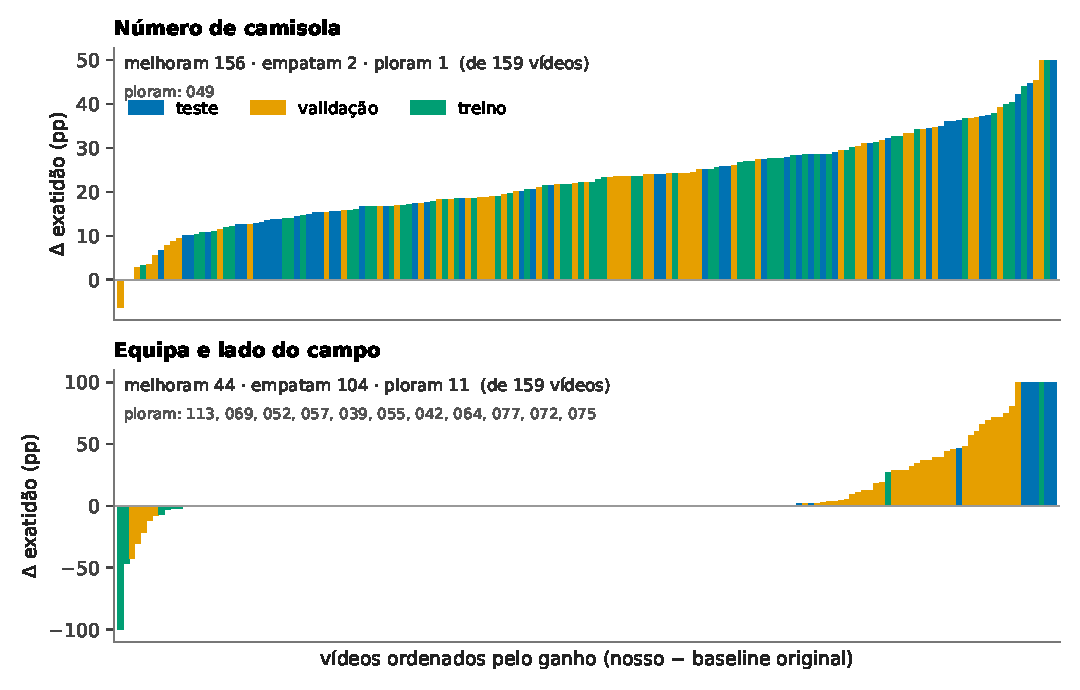
\includegraphics[width=\textwidth]{fig_delta_por_video.pdf}
    \caption{Diferença de exatidão por vídeo entre o sistema proposto e a solução de referência, para o número de camisola (em cima) e para a equipa e lado do campo (em baixo), nos $159$ vídeos ordenados pelo ganho e coloridos por subconjunto.}
    \label{fig:delta-video}
\end{figure}

A inspeção visual dá a mesma imagem por outro ângulo (Tabela~\ref{tab:visual}). Na solução de referência, $111$ dos $159$ vídeos estão corretos. Os restantes repartem-se por lado trocado ($7$), agrupamento colapsado numa só equipa ($7$), agrupamento misturado ($14$) e uma equipa inteira classificada como equipa de arbitragem ($20$). No sistema proposto, $132$ vídeos estão corretos, e as falhas do módulo de equipa propriamente dito descem de $28$ para $7$. Ficam $3$ com o lado trocado, $1$ com o agrupamento colapsado e $3$ com um \emph{tracklet} isolado na equipa errada. A Figura~\ref{fig:frames-148} ilustra uma das falhas da referência, o lado trocado, com o mesmo instante do vídeo SNGS-148 nos dois sistemas.

\begin{table}[htbp]
    \centering
    \caption{Inspeção visual dos $159$ vídeos de cada sistema, por categoria de erro. A última coluna conta os vídeos em que o sistema está correto e é a anotação de referência que está invertida, e esses contam também na coluna dos corretos. Os veredictos da solução de referência foram revistos após a recalibração descrita na Secção~\ref{sec:res_calib_defeito}, que alterou o resultado em oito vídeos.}
    \label{tab:visual}
    \begin{tabular}{|l|c|c|c|c|c|c|}
        \hline
        \textbf{Sistema} & \textbf{Correto} & \textbf{Lado trocado} & \textbf{Colapsado} & \textbf{Misturado} & \textbf{Função} & \textbf{Anot.\ invertida} \\
        \hline
        Referência & $111$ & $7$ & $7$ & $14$ & $20$ & $5$ \\
        \hline
        Proposto   & $132$ & $3$ & $1$ & $3$ & $20$ & $4$ \\
        \hline
    \end{tabular}
\end{table}

\begin{figure}[htbp]
    \centering
    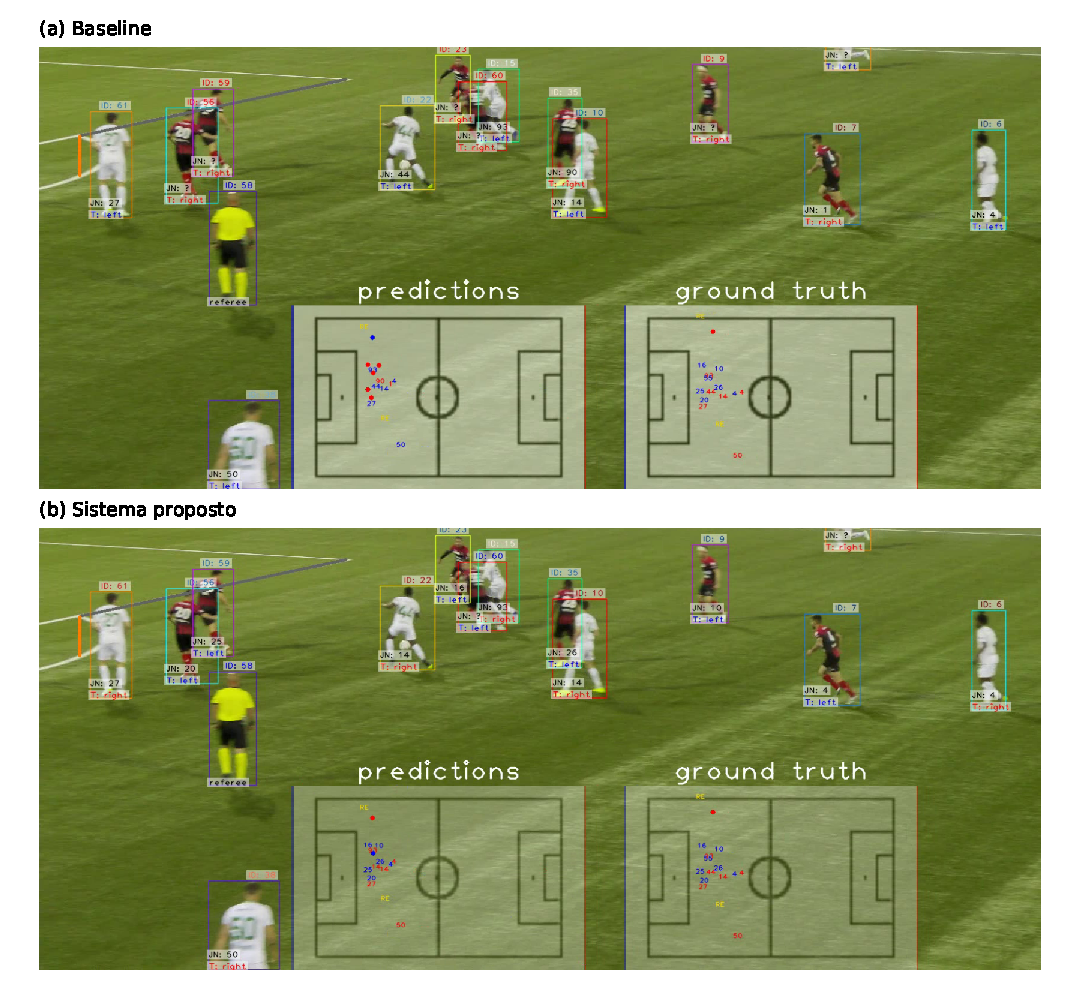
\includegraphics[width=\textwidth]{fig_frames_148.pdf}
    \caption{O mesmo instante do vídeo SNGS-148 nos dois sistemas. Nos mapas do campo, à esquerda as predições e à direita a anotação de referência. A solução de referência atribui a cada equipa o lado oposto ao real, o sistema proposto acerta.}
    \label{fig:frames-148}
\end{figure}

A categoria \emph{função} merece uma nota à parte. Nos $20$ vídeos de validação SNGS-039 a SNGS-058, uma das equipas joga de amarelo e o classificador de função da solução de referência, que este trabalho não alterou, classifica-a como equipa de arbitragem nos dois sistemas. Os \emph{tracklets} dessa equipa saem do agrupamento antes de ele começar, e a equipa e o lado ficam mal à partida. Trata-se de uma falha comum, exterior aos módulos intervencionados, e é o principal motivo de a validação ficar abaixo dos outros dois conjuntos nas Tabelas~\ref{tab:team-conjuntos} e~\ref{tab:gshota}.

\subsection{A Auditoria de Partições Degeneradas}\label{sec:res_equipa_degenerada}

Uma versão anterior deste sistema apresentava uma falha própria, que importa expor porque explica a verificação que hoje o módulo faz. Em onze vídeos o agrupamento terminava com quase todos os jogadores no mesmo grupo, o que equivale a afirmar que todos os que estão em campo pertencem à mesma equipa. A partição era de tal forma desequilibrada que o grupo menor reunia entre $0.1\%$ e $7.8\%$ das deteções de jogadores, ao passo que nos restantes $148$ vídeos nunca desce abaixo de $8.7\%$ e fica tipicamente perto de metade. O erro resultante não era aleatório, uma vez que em nove desses onze vídeos a exatidão situava-se entre $44\%$ e $61\%$, isto é, ao nível de atribuir as equipas por sorteio. Os dois restantes são extremos do mesmo problema, com a atribuição toda errada num caso e toda certa no outro, esta última por a cascata do lado ter acertado no grupo dominante.

A separação entre os dois casos é nítida e dispensa a anotação, pelo que pode ser verificada pelo próprio módulo em tempo de execução. Acrescentou-se por isso uma terceira verificação à auditoria da Secção~\ref{sec:agrupamento}. Quando o grupo menor fica abaixo de $8\%$ das deteções de jogadores, a partição é rejeitada e os \emph{tracklets} são reagrupados pela cor do equipamento, medida diretamente nos \emph{frames} originais através de um histograma no espaço HSV da região do tronco, com os píxeis de relva excluídos. O reagrupamento só é aceite se ele próprio produzir dois grupos equilibrados, sob pena de se trocar uma partição degenerada por outra.

O reagrupamento está sujeito a duas salvaguardas, ambas necessárias. A primeira exige que a partição de resgate passe o mesmo teste que reprovou a anterior, medido nas deteções e não apenas nos \emph{tracklets}, pois um resgate pode ser equilibrado em número de \emph{tracklets} e continuar a concentrar as deteções num só grupo. A segunda recusa o reagrupamento quando o classificador de função dá como arbitragem mais de um quarto dos \emph{tracklets} que dá como jogador. Nesse caso falta ao agrupamento uma equipa inteira, e separar por cor o que resta apenas parte uma equipa ao meio, produzindo um resultado que a métrica premeia ligeiramente mas que a inspeção visual mostra não ter sentido.

A Tabela~\ref{tab:regressoes} mostra o efeito da verificação nos onze vídeos em que ela dispara. Em oito o reagrupamento é aceite e em sete deles o agrupamento passa a estar inteiramente correto. Nos outros três é recusado pelas salvaguardas, e esses vídeos mantêm exatamente o resultado que já tinham. Em nenhum dos $148$ restantes a verificação chega a ser acionada.

\begin{table}[htbp]
    \centering
    \caption{Vídeos em que a verificação de partições degeneradas dispara. A coluna do grupo menor refere-se à partição rejeitada. As três últimas dão a exatidão da equipa na solução de referência, no sistema proposto antes da verificação e depois dela.}
    \label{tab:regressoes}
    \begin{tabular}{|l|c|c|c|c|c|}
        \hline
        \textbf{Vídeo} & \textbf{Grupo menor} & \textbf{Grupos após} & \textbf{Referência} & \textbf{Antes} & \textbf{Depois} \\
        \hline
        SNGS-025 & $3.9\%$ & $33/46$ & $100.0\%$ & $61.4\%$ & $100.0\%$ \\
        \hline
        SNGS-027 & $2.8\%$ & $37/40$ & $52.2\%$ & $47.8\%$ & $100.0\%$ \\
        \hline
        SNGS-028 & $5.9\%$ & $26/27$ & $54.5\%$ & $54.5\%$ & $100.0\%$ \\
        \hline
        SNGS-030 & $0.5\%$ & $31/14$ & $40.0\%$ & $60.0\%$ & $100.0\%$ \\
        \hline
        SNGS-036 & $3.3\%$ & $19/24$ & $96.8\%$ & $51.6\%$ & $100.0\%$ \\
        \hline
        SNGS-038 & $0.1\%$ & $28/16$ & $100.0\%$ & $55.2\%$ & $100.0\%$ \\
        \hline
        SNGS-091 & $7.8\%$ & $33/37$ & $86.7\%$ & $57.8\%$ & $97.8\%$ \\
        \hline
        SNGS-131 & $7.1\%$ & $29/40$ & $0.0\%$ & $43.6\%$ & $0.0\%$ \\
        \hline
        \multicolumn{6}{|l|}{\emph{Reagrupamento recusado pelas salvaguardas}} \\
        \hline
        SNGS-039 & $5.8\%$ & --- & $21.9\%$ & $0.0\%$ & $0.0\%$ \\
        \hline
        SNGS-050 & $0.8\%$ & --- & $60.9\%$ & $100.0\%$ & $100.0\%$ \\
        \hline
        SNGS-069 & $2.7\%$ & --- & $100.0\%$ & $53.3\%$ & $53.3\%$ \\
        \hline
    \end{tabular}
\end{table}

Os casos que não se resolvem dizem, cada um, algo distinto. No SNGS-039 e no SNGS-050 a equipa que falta é a de amarelo, dada como arbitragem pelo classificador de função, e é a segunda salvaguarda que impede o módulo de agir sobre uma entrada incompleta. No SNGS-069, o único em que a cor não chega, as equipas jogam de verde e de branco e a exclusão dos píxeis de relva, que é o que torna o descritor robusto em todos os outros vídeos, remove também parte das camisolas verdes, pelo que o resgate volta a concentrar as deteções num só grupo e é recusado pela primeira salvaguarda. Uma máscara estimada a partir do fundo local, em vez de um intervalo fixo de tom, resolveria o caso e fica registada como trabalho imediato. O SNGS-131 é o mais instrutivo. O agrupamento passa a estar correto, como a inspeção visual confirma, mas a anotação de referência atribui a cada equipa o lado oposto ao que ocupa, pelo que a métrica passa de $43.6\%$ para zero precisamente por o sistema ter deixado de errar. Este caso analisa-se na Secção~\ref{sec:res_equipa_metrica}.

\subsection{Regressões Remanescentes}\label{sec:res_equipa_regressoes}

Nos $11$ vídeos em que a métrica ainda dá o sistema proposto abaixo da referência, $5$ pertencem ao bloco da equipa de amarelo, onde a métrica é calculada sobre a equipa que sobra, outro é o SNGS-113, com o lado trocado, outro é o SNGS-069, acima descrito, e os restantes diferem da referência em um ou dois \emph{tracklets}.

Os vídeos com o lado trocado têm outra natureza. No SNGS-113 os dois grupos estão bem separados mas o lado está trocado. A votação relativa, segundo critério da cascata, decide por uma margem de $15$ pontos num vídeo em que as duas equipas ocupam a mesma metade do campo, enquanto a média das posições, que a referência usa e que teria acertado, nunca chega a ser consultada. O caso foi analisado em detalhe na Secção~\ref{sec:mapeamento}. No SNGS-106 o lado está trocado nos dois sistemas. O terceiro caso é o SNGS-197, discutido na secção seguinte, em que o lado atribuído coincide com o da anotação invertida e a métrica, por isso, não o penaliza. Os três vídeos com agrupamento misturado (SNGS-023, SNGS-156 e SNGS-187) têm um único \emph{tracklet} na equipa errada e a métrica, como se explica a seguir, não o regista.

\subsection{O Que a Métrica Não Vê}\label{sec:res_equipa_metrica}

A confrontação entre a métrica e a inspeção visual revela três pontos cegos que ficam aqui documentados, porque condicionam a leitura de qualquer resultado desta tarefa.

O primeiro é que a exatidão da equipa é calculada apenas sobre os \emph{tracklets} classificados como jogadores ou guarda-redes. Quando um \emph{tracklet} de jogador é classificado como árbitro, deixa de contar, e um vídeo em que uma equipa inteira desaparece para a arbitragem pode apresentar uma exatidão de equipa elevada calculada sobre a equipa que sobrou. Os três vídeos com um \emph{tracklet} na equipa errada estão nesta situação, com $100\%$ na métrica.

O segundo ponto cego são as trocas de identidade. Um \emph{tracklet} que siga dois jogadores diferentes ao longo do vídeo é excluído da contagem, porque não há uma equipa de referência única com que o comparar. A exclusão é metodologicamente correta, mas retira da avaliação precisamente os casos em que o seguimento falhou, e não é residual. No SNGS-030, por exemplo, dos $38$ \emph{tracklets} emparelhados com a anotação apenas $20$ são avaliados, e um dos excluídos, que a inspeção visual assinala como tendo a equipa errada, segue um jogador em metade dos \emph{frames} e outro na outra metade. Um vídeo pode assim apresentar $100\%$ de exatidão e mostrar, no vídeo renderizado, um jogador com a cor trocada.

O terceiro é a anotação de referência. Em cinco vídeos (SNGS-126, SNGS-131 e SNGS-197 no teste, SNGS-092 na validação e SNGS-111 no treino), a inspeção visual mostra que os lados anotados estão invertidos em relação ao que se vê no vídeo, e um sistema que acerte recebe $0\%$. A afirmação tem correspondência na própria anotação. Nos cinco vídeos, a posição média no campo dos jogadores anotados como equipa da esquerda está mais à direita do que a dos anotados como equipa da direita, com diferenças entre $3.8$ e $8.8$ metros. O mesmo teste, aplicado aos $160$ vídeos, assinala mais dois casos, o SNGS-038 e o SNGS-195, mas com diferenças de $1.0$ e $0.7$ metros, valores que uma única fase de ataque explica e que a inspeção visual não confirmou. O critério posicional isolado não é, portanto, prova suficiente, e é a inspeção visual que separa os cinco casos dos dois. A observação é consistente com a nota de \citet{oo2026broadcast2pitch}, que assinala SNGS-126, SNGS-131 e SNGS-197 como incorretamente anotados no atributo equipa, e acrescenta-lhe dois vídeos, um da validação e outro do treino, que aquele trabalho não podia observar por avaliar apenas o conjunto de teste. O efeito nas tabelas é o de premiar quem erra, nos dois sentidos. O SNGS-131 ilustra um deles. A solução de referência agrupa as duas equipas corretamente e, por isso mesmo, recebe $0\%$. O sistema proposto, enquanto colapsava o agrupamento, recebia $43.6\%$, porque metade dos \emph{tracklets} calhava do lado que a anotação indica, e ao passar a agrupar corretamente desceu também a zero. O SNGS-197 ilustra o sentido inverso. Aí é o sistema proposto que reproduz a inversão da anotação e recebe $100\%$, ao passo que a solução de referência, que atribui os lados como se vê no vídeo, recebe zero. Por isso esse vídeo conta como lado trocado na inspeção visual do sistema proposto, apesar de a métrica lhe dar a pontuação máxima. Estes casos foram mantidos nas tabelas tal como a métrica os conta, contra a anotação publicada, para que os valores sejam comparáveis com os de outros trabalhos. Excluindo os cinco, a exatidão da equipa do sistema proposto sobre os restantes $154$ vídeos avaliados sobe de $92.8\%$ para $95.2\%$.

\subsection{Contributo de Cada Alteração}\label{sec:res_equipa_ablacao}

Durante o desenvolvimento, as alterações ao módulo foram introduzidas uma de cada vez e medidas sobre os $39$ vídeos de teste para os quais existia então uma referência de comparação (Tabela~\ref{tab:team-resultados}). A correção do agrupamento e a cascata de votação respondem pela quase totalidade do ganho, ao recuperarem vídeos em que a média simples da referência falhava por completo. O desempate pela deriva do guarda-redes recupera o último vídeo, cujas posições médias eram indistinguíveis. A verificação de partições degeneradas é posterior a esta série de experiências e o seu contributo é medido separadamente na Secção~\ref{sec:res_equipa_degenerada}, sobre a totalidade dos $159$ vídeos.

\begin{table}[htbp]
    \centering
    \caption{Contributo incremental de cada alteração para a atribuição da equipa e do lado do campo, medido durante o desenvolvimento sobre $39$ vídeos do conjunto de teste.}
    \label{tab:team-resultados}
    \begin{tabular}{|l|c|c|}
        \hline
        \textbf{Estado do sistema} & \textbf{Exatidão} & \textbf{$\Delta$} \\
        \hline
        Solução de referência                              & $85.4\%$ ($1499/1755$) & --- \\
        \hline
        + agrupamento com auditoria e cascata de votação   & $96.1\%$ ($1686/1755$) & $+10.7$ pp \\
        \hline
        + desempate pela deriva do guarda-redes            & $97.8\%$ ($1717/1755$) & $+1.7$ pp \\
        \hline
    \end{tabular}
\end{table}

\subsection{Robustez do Critério de Atribuição do Lado}\label{sec:res_lado_quantificacao}

Como se referiu na Secção~\ref{sec:equipa-desafio}, a generalidade das soluções apresentadas ao desafio decide o lado do campo comparando a posição horizontal média dos dois grupos de jogadores, e nenhuma quantifica com que frequência essa suposição falha. Essa medição foi feita neste trabalho diretamente sobre a anotação de referência dos $160$ vídeos, de modo a caracterizar o critério independentemente dos erros do \emph{pipeline}.

O procedimento assenta em dois testes. O primeiro usa o guarda-redes como referência, uma vez que, ao contrário dos jogadores de campo, não acompanha as fases de ataque, e verifica se a sua posição é compatível com o lado atribuído à sua equipa. O segundo compara a posição mediana dos jogadores de cada equipa e assinala os vídeos em que a ordem se inverte. Os resultados constam da Tabela~\ref{tab:lado-inversoes}. A posição do guarda-redes nunca contradiz a anotação nos $155$ vídeos em que existe guarda-redes observável, ao passo que o critério posicional se inverte em $9$ dos $160$ vídeos, ou seja em $5.6\%$ dos casos. Usou-se a mediana por ser menos sensível a um jogador isolado no meio-campo adversário. Com a média simples, que é a formulação habitual na literatura, a ordem inverte-se em sete vídeos.

\begin{table}[htbp]
    \centering
    \caption{Comportamento dos dois critérios de atribuição do lado do campo, medido sobre a anotação de referência dos três subconjuntos.}
    \label{tab:lado-inversoes}
    \begin{tabular}{|l|c|c|}
        \hline
        \textbf{Critério} & \textbf{Vídeos avaliáveis} & \textbf{Casos em que falha} \\
        \hline
        Posição do guarda-redes  & $155$ & $0$ \\
        \hline
        Posição média da equipa  & $160$ & $9$ ($5.6\%$) \\
        \hline
    \end{tabular}
\end{table}

A inversão ocorre em situações de pressão prolongada, em que a equipa atacante se instala no meio-campo adversário e a sua posição média passa a estar do lado que não lhe corresponde. É precisamente este cenário que motiva a cascata de critérios da Secção~\ref{sec:mapeamento}, em vez de um critério único. Ensaiou-se ainda um critério alternativo, o de substituir a posição média pelo jogador de campo mais recuado, partindo da ideia de que a última linha defensiva se mantém entre os atacantes e a sua própria baliza. Avaliado sobre a anotação de referência, este critério acerta em apenas $68.6\%$ dos vídeos, contra $94.4\%$ da posição média, e falha nos nove casos difíceis. A causa é o enquadramento televisivo, uma vez que a câmara mostra apenas parte do campo e o jogador mais recuado visível não é necessariamente o último defesa. A alternativa foi, por isso, descartada.

\section{Desempenho Global}\label{sec:desempenho_global}\label{sec:desempenho-global}

O efeito das alterações no sistema completo é medido pelo GS-HOTA, calculado com a implementação oficial sobre cada subconjunto inteiro. Antes dos valores, é necessário dar conta de uma condição da comparação que só a avaliação global tornou visível.

\subsection{Um Defeito de Calibração na Solução de Referência}\label{sec:res_calib_defeito}

Como a deteção, o seguimento e a calibração são idênticos nos dois sistemas, o GS-HOTA calculado apenas com a posição, sem qualquer atributo, deveria ser o mesmo. Não era. A primeira avaliação deu $56.7\%$ para a referência e $61.8\%$ para o sistema proposto no conjunto de teste. A comparação das posições projetadas no campo, deteção a deteção, mostrou que coincidem exatamente em um de cada oito \emph{frames} e diferem, tipicamente entre um e quatro metros, nos restantes. A origem está na configuração por omissão da solução de referência, que processa a calibração em lotes de oito \emph{frames}, de tal modo que o módulo que estima a homografia lê os pontos do campo do primeiro \emph{frame} de cada lote e aplica a homografia resultante aos outros sete. O sistema proposto, por limitações de memória gráfica, calibrava um \emph{frame} de cada vez e não sofria do defeito.

Para que a comparação isole o que foi alterado, a solução de referência foi recalibrada \emph{frame} a \emph{frame}, a partir dos pontos do campo já estimados, e o lado de cada equipa foi recalculado com o módulo original sobre as posições corrigidas. Todos os valores da referência reportados neste capítulo, incluindo os das Secções~\ref{sec:res_jnr} e~\ref{sec:res_equipa}, dizem respeito a esta versão corrigida. O defeito é da solução distribuída pelos organizadores e vale, sozinho, cerca de $5$ pontos de GS-HOTA calculado apenas com a posição e $2.4$ pontos na métrica completa, na sua configuração por omissão.

\subsection{GS-HOTA por Subconjunto}\label{sec:res_gshota}

A Tabela~\ref{tab:gshota} apresenta o GS-HOTA dos dois sistemas nos três subconjuntos, com as componentes de deteção (DetA), de associação (AssA) e de localização (LocA). O sistema proposto obtém $47.87\%$ no teste, $36.79\%$ na validação e $45.37\%$ no treino, contra $31.30\%$, $23.68\%$ e $31.52\%$ da referência corrigida, ou seja, ganhos de $16.6$, $13.1$ e $13.8$ pontos. A dispersão entre conjuntos é, em ambos os sistemas, maior do que a diferença entre teste e treino, e o ganho no conjunto de treino, que não interveio no desenvolvimento, é da mesma ordem do obtido no teste. Não há indício de que o desempenho resulte de sobreajuste aos dados sobre os quais os limiares foram afinados.

\begin{table}[htbp]
    \centering
    \caption{GS-HOTA e componentes nos três subconjuntos anotados, calculados com a implementação oficial sobre cada subconjunto inteiro. A referência é a solução original recalibrada \emph{frame} a \emph{frame} (Secção~\ref{sec:res_calib_defeito}).}
    \label{tab:gshota}
    \begin{tabular}{|l|l|c|c|c|c|}
        \hline
        \textbf{Conjunto} & \textbf{Sistema} & \textbf{GS-HOTA} & \textbf{DetA} & \textbf{AssA} & \textbf{LocA} \\
        \hline
        Teste & Referência & $31.30\%$ & $17.5$ & $56.1$ & $92.8$ \\
        \hline
         & Proposto & $47.87\%$ & $39.0$ & $58.7$ & $93.3$ \\
        \hline
        Validação & Referência & $23.68\%$ & $10.3$ & $54.4$ & $91.5$ \\
        \hline
         & Proposto & $36.79\%$ & $24.5$ & $55.3$ & $92.3$ \\
        \hline
        Treino & Referência & $31.52\%$ & $17.9$ & $55.6$ & $92.0$ \\
        \hline
         & Proposto & $45.37\%$ & $36.3$ & $56.7$ & $92.2$ \\
        \hline
    \end{tabular}
\end{table}

Por vídeo, o ganho mediano de GS-HOTA é de $+15.0$ pontos no teste, $+15.5$ na validação e $+14.0$ no treino. Os vídeos em que o sistema proposto fica abaixo da referência por mais de um ponto são 6 (SNGS-039, SNGS-042, SNGS-043, SNGS-049, SNGS-069, SNGS-113), e coincidem com as regressões da Secção~\ref{sec:res_equipa_regressoes}.

\subsection{Decomposição por Atributo}\label{sec:res_decomposicao}

O GS-HOTA anula a similaridade entre uma deteção e a anotação sempre que a função, a equipa ou o número não coincidem, pelo que agrega, num único valor, o contributo de todos os módulos. Para separar o que cabe a cada um, a métrica foi recalculada com os atributos ativados de forma progressiva, primeiro apenas com a posição no campo, depois com a função, a equipa e o número de camisola, para os dois sistemas (Tabela~\ref{tab:decomposicao} e Figura~\ref{fig:decomposicao}). É um procedimento análogo ao com que a solução vencedora da edição de 2025 caracterizou o seu próprio sistema (Secção~\ref{sec:metricas}), com duas diferenças, a de os atributos serem aqui acrescentados de forma cumulativa, pelo que a última coluna é a métrica oficial, e a de ser aplicado aos dois sistemas em comparação.

\begin{table}[htbp]
    \centering
    \caption{GS-HOTA com os atributos ativados de forma progressiva. Cada coluna acrescenta um atributo à anterior. A última coluna é a métrica oficial.}
    \label{tab:decomposicao}
    \begin{tabular}{|l|l|c|c|c|c|}
        \hline
        \textbf{Conjunto} & \textbf{Sistema} & \textbf{Posição} & \textbf{+ função} & \textbf{+ equipa} & \textbf{+ número} \\
        \hline
        Teste & Referência & $61.8$ & $59.4$ & $53.8$ & $31.3$ \\
        \hline
         & Proposto & $61.8$ & $59.4$ & $57.4$ & $47.9$ \\
        \hline
        Validação & Referência & $57.7$ & $47.4$ & $38.5$ & $23.7$ \\
        \hline
         & Proposto & $57.7$ & $47.4$ & $43.0$ & $36.8$ \\
        \hline
        Treino & Referência & $58.3$ & $58.2$ & $56.1$ & $31.5$ \\
        \hline
         & Proposto & $58.3$ & $58.2$ & $55.8$ & $45.4$ \\
        \hline
    \end{tabular}
\end{table}

\begin{figure}[htbp]
    \centering
    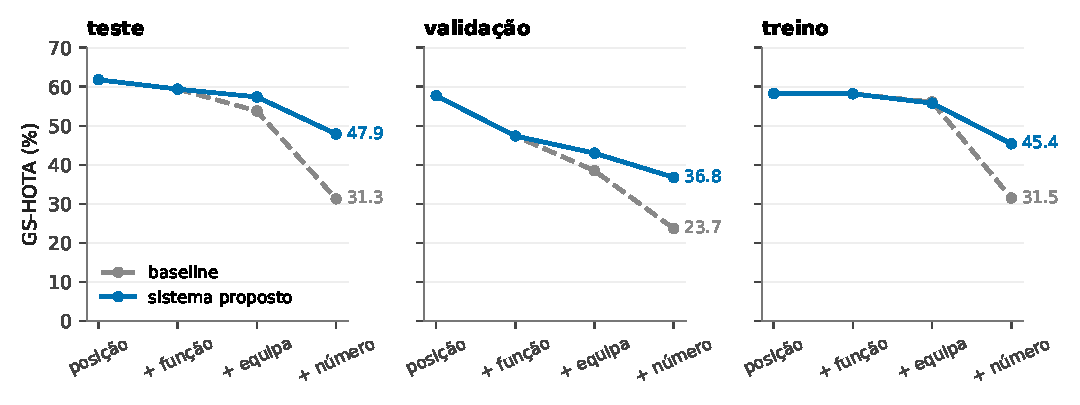
\includegraphics[width=\textwidth]{fig_decomposicao_gshota.pdf}
    \caption{GS-HOTA à medida que se ativam os atributos, nos três subconjuntos. A distância entre pontos consecutivos é o custo de cada atributo. A distância entre as duas linhas, o ganho do sistema proposto.}
    \label{fig:decomposicao}
\end{figure}

A leitura é direta. Com a posição apenas, os dois sistemas coincidem, como têm de coincidir, e o valor obtido, entre $57.7\%$ e $61.8\%$, é o teto que a deteção, o seguimento e a calibração, mantidos intactos, impõem a tudo o que vem depois. A função, que também não foi alterada, custa o mesmo aos dois sistemas, e custa muito mais na validação, $10.3$ pontos, do que no teste e no treino, $2.4$ e $0.1$, que é a assinatura dos vinte vídeos da equipa de amarelo. Os dois atributos alterados são os que separam as linhas. Na referência, a equipa custa $5.6$ pontos no teste e o número $22.5$, ao passo que no sistema proposto custam $2.0$ e $9.5$. Do ganho total de $16.6$ pontos no teste, $3.6$ vêm da equipa e $12.9$ do número. Na validação, dos $13.1$ pontos, $4.6$ vêm da equipa e $8.6$ do número. No treino, dos $13.8$, a equipa não contribui ($-0.2$) e $14.1$ vêm do número. O número de camisola é, nos dois sistemas e nos três conjuntos, o atributo que mais custa, com uma única exceção, na validação do sistema proposto, onde a função, pelos vinte vídeos da equipa de amarelo, custa mais do que o número ($10.3$ contra $6.2$ pontos), o que confirma, com a métrica oficial e sobre a solução de referência, o diagnóstico que a solução vencedora de 2025 fez sobre a sua.

\subsection{Enquadramento Competitivo}\label{sec:res_leaderboard}

Para situar estes valores, a Tabela~\ref{tab:leaderboard} reúne os três melhores sistemas e a solução de referência de cada edição do desafio, apurados no conjunto de \emph{challenge}, de anotações reservadas e distinto dos conjuntos usados neste trabalho. A referência oficial da edição de 2025 obtém $29.01\%$ nesse conjunto. A mesma solução, executada por nós na sua configuração por omissão, obtém $28.95\%$ no conjunto de teste, o que dá alguma confiança na reprodução. Os sistemas no topo ultrapassam os $60\%$, otimizando a totalidade do \emph{pipeline}, incluindo a deteção e a calibração, precisamente as componentes que este trabalho manteve intactas e que, pela Tabela~\ref{tab:decomposicao}, limitam o sistema proposto a um teto de cerca de $62$ pontos no conjunto de teste antes de qualquer atributo ser considerado.

\begin{table}[htbp]
    \centering
    \caption{Três melhores sistemas e solução de referência das edições de 2024 e 2025 do desafio, apurados no conjunto de \emph{challenge}. Valores da avaliação oficial.}
    \label{tab:leaderboard}
    \begin{tabular}{|l|c|}
        \hline
        \textbf{Sistema} & \textbf{GS-HOTA} \\
        \hline
        \multicolumn{2}{|l|}{\textit{Edição de 2024}} \\
        \hline
        Constructor Tech  & $63.81\%$ \\
        \hline
        UPCxMobius        & $43.15\%$ \\
        \hline
        JAM               & $34.40\%$ \\
        \hline
        Referência oficial & $23.36\%$ \\
        \hline
        \multicolumn{2}{|l|}{\textit{Edição de 2025}} \\
        \hline
        KIST-GSR          & $63.90\%$ \\
        \hline
        Constructor Tech  & $63.81\%$ \\
        \hline
        lianyou           & $62.76\%$ \\
        \hline
        Referência oficial & $29.01\%$ \\
        \hline
    \end{tabular}
\end{table}

As escolhas de conceção deste trabalho coincidem, em dois pontos, com as dessas soluções. A vencedora de 2025 formula a identificação como uma tarefa multimodal resolvida por um modelo de visão e linguagem, o mesmo tipo de modelo aqui adotado para a leitura do número, e determina a equipa por agrupamento da cor do equipamento combinado com a posição no campo, à semelhança do módulo de atribuição. O passo de recorte da região dorsal guiado pela pose, que precede a leitura, não consta das descrições publicadas dessas soluções.

\section{Custo Computacional}\label{sec:res_tempos}

A Tabela~\ref{tab:tempos} apresenta o tempo de execução de cada módulo, medido no motor de execução para cada vídeo de $30$ segundos ($750$ \emph{frames}), na GPU portátil descrita na Secção~\ref{sec:ambiente}. Os módulos alterados têm um custo residual. O agrupamento e o lado do campo somam menos de dois segundos por vídeo nos dois sistemas, e o leitor proposto, apesar de ser um modelo de visão e linguagem, demora o mesmo que o MMOCR que substitui, porque só lê os recortes que passam o filtro de qualidade. A diferença na calibração, de $5.7$ para $21.5$ segundos, é o custo de calibrar todos os \emph{frames} em vez de um em cada oito (Secção~\ref{sec:res_calib_defeito}). O tempo total, cerca de $21$ minutos por vídeo, é dominado pela reidentificação, pela leitura do número e pela estimativa dos pontos do campo, e situa-se muito longe do tempo real. A redução deste custo é discutida no Capítulo~\ref{cap:conclusao}.

\begin{table}[htbp]
    \centering
    \caption{Tempo de execução por módulo e por vídeo de $30$ segundos, mediana sobre os vídeos processados (segundos). O sistema proposto foi medido com menos processos de carregamento de dados e memória mais apertada, o que explica parte da diferença na reidentificação e na leitura.}
    \label{tab:tempos}
    \begin{tabular}{|l|c|c|}
        \hline
        \textbf{Módulo} & \textbf{Referência} & \textbf{Proposto} \\
        \hline
        Deteção (YOLOv8)                          & $97.3$  & $96.4$ \\
        \hline
        Reidentificação (PRTReID)                 & $448.7$ & $484.4$ \\
        \hline
        Seguimento (StrongSORT)                   & $31.8$  & $30.9$ \\
        \hline
        Pontos do campo (NBJW)                    & $211.9$ & $210.3$ \\
        \hline
        Calibração (homografia)                   & $5.7$   & $21.5$ \\
        \hline
        Número de camisola (MMOCR / proposto)     & $486.7$ & $477.7$ \\
        \hline
        Voto por \emph{tracklet}                  & $0.1$   & $0.1$ \\
        \hline
        Equipa (agrupamento)                      & $0.7$   & $1.3$ \\
        \hline
        Lado do campo                             & $0.0$   & $0.1$ \\
        \hline
        Total dos módulos                         & $21.3$ min & $22.0$ min \\
        \hline
    \end{tabular}
\end{table}

A decisão pela confiança da leitura acrescenta a este tempo uma segunda leitura de cada janela, com registo das probabilidades dos \emph{tokens}, que custa cerca de quatro minutos por vídeo. Como essas probabilidades são produzidas na mesma chamada ao modelo que gera a resposta, podem ser registadas logo na primeira leitura, o que elimina este custo adicional numa implementação integrada.

\section{Síntese}\label{sec:res_sintese}

Os resultados mostram que uma intervenção concentrada em quatro dos nove módulos, três deles substituídos ou reescritos e um estendido, melhora de forma clara e consistente o desempenho global. O reconhecimento do número mais do que duplica face à referência, de $15.3\%$ para $42.6\%$ sobre $159$ vídeos, com melhoria em $156$ deles e nenhuma regressão, e a decisão pela confiança da leitura reduz os números errados a cerca de um terço. A atribuição da equipa e do lado passa de $83.5\%$ para $92.8\%$, e o número de vídeos com o módulo de equipa em falha desce de $28$ para $7$. O GS-HOTA sobe $16.6$ pontos no teste, $13.1$ na validação e $13.8$ no treino, e a decomposição por atributo imputa esse ganho, na totalidade, aos dois atributos alterados.

A avaliação sobre os três subconjuntos acrescenta duas garantias. O conjunto de treino, que não interveio em nenhuma decisão de conceção, produz ganhos da mesma ordem dos do teste, e a comparação é feita contra a solução de referência corrigida de um defeito de calibração que, na configuração distribuída, lhe custa cerca de $5$ pontos na posição e $2.4$ na métrica completa, e que inflacionaria o ganho reclamado.

Os limites ficaram igualmente delimitados. No número, as experiências controladas mostram que nenhuma transformação da imagem cria informação onde ela não existe, e que o erro restante se deve sobretudo a recortes sem resolução e a trocas de identidade do seguimento, que estão fora do âmbito do módulo. Na equipa, a inspeção visual mostrou que ficam vinte vídeos em que o classificador de função, não alterado, retira uma equipa inteira do agrupamento, e três com o lado trocado, um deles comum aos dois sistemas. A falha que era própria deste trabalho, a aceitação de partições degeneradas, encontra-se corrigida pela verificação descrita na Secção~\ref{sec:res_equipa_degenerada}, que a resolve em sete dos onze vídeos afetados sem alterar nenhum dos restantes $148$.
